% Generated from paper/source. Do not edit by hand.
\section{Results}
\subsection{Comparator identity changes the conclusion}
The historical within-NeuroWorld comparison is positive: complex minus two-channel real at moderate shift is +0.0602 top-1. The stronger comparisons are all non-positive. The QN-000031 power pilot estimates -0.0552 at size 1,000. Reduced discovery estimates -0.0370 against the cellwise best-real envelope. Held-out reduced confirmation estimates -0.00916. These values arise from different task surfaces and are not combined as a meta-analysis. Their joint role is diagnostic: the sign of the conclusion depends on which real comparator and task family are named.

\subsection{Exact real computation reproduces the candidate}
In the held-out study, complex and exact-real top-1 accuracies match in every one of 1,920 nested cells. Maximum absolute differences are 0 for top-1, 3.58 x 10\textasciicircum{}-7 for NLL, and 1.19 x 10\textasciicircum{}-7 for ECE. The earlier mapped mechanism experiment found maximum metric disagreement of approximately 4.8 x 10\textasciicircum{}-7. This replication across four new generator families supports implementation-level equivalence at numerical precision.

The exact-real control wins the best-real selection in 1,478 held-out cells, while the real polar operator wins 442. The complex operator wins none. Because the exact block is constrained to the same mapped structure, these results do not show that an unrestricted real model is inherently better. They show that explicitly complex arithmetic is not required to obtain the candidate's computation and does not create a favorable top-1 effect in the tested training pipeline.

\subsection{Reduced discovery yields no positive effects}
Across 2,880 nested discovery effects, zero are positive and the mean is -0.03695. The result spans four generator families, two training sizes, five training seeds, 24 worlds, and three severities. It is outcome-ineligible because only five models and one search configuration per model were executed. Nevertheless, it provides no empirical basis for advancing an intrinsic complex-advantage claim.

Six structural relationship families were fit to 12 family-by-severity aggregates. The quadratic candidate minimized the prespecified selection proxy, with discovery R2 0.9487 and MAE 0.002604. Its predictors were empirical order-target mutual information and shift severity. The frozen artifact explicitly prohibited a general-law claim and use for the grand outcome.

\subsection{The frozen relationship fails untouched families}
Held-out evaluation contains 1,920 nested effects. Zero are positive, 1,538 are exactly zero at the recorded precision, and the remaining 382 are negative. The mean is -0.009158, median 0, standard deviation 0.02355, 10\% trimmed mean -0.002485, and worst-decile mean -0.04167. Across 128 world summaries, the mean is again -0.009158 and the median is -0.008056.

The hierarchical bootstrap interval is -0.01325 to -0.00457. The exploratory two-sided world sign-flip p value is approximately 5.0 x 10\textasciicircum{}-6. Because the profile is outcome-ineligible, this p value cannot promote the study into the preregistered grand category. It instead quantifies the consistency of a non-positive effect within the executed scope.

The frozen quadratic relationship transfers only the sign. Held-out sign accuracy is 1.0 because both predicted and observed aggregates are non-positive. Magnitude prediction fails: R2 is -30.94 and MAE is 0.03126, violating the frozen R2 and MAE thresholds. No coefficients were changed after this result. QN-LAW-001 is therefore a failed candidate, not a general computational law.

\begin{figure}[t]
\centering
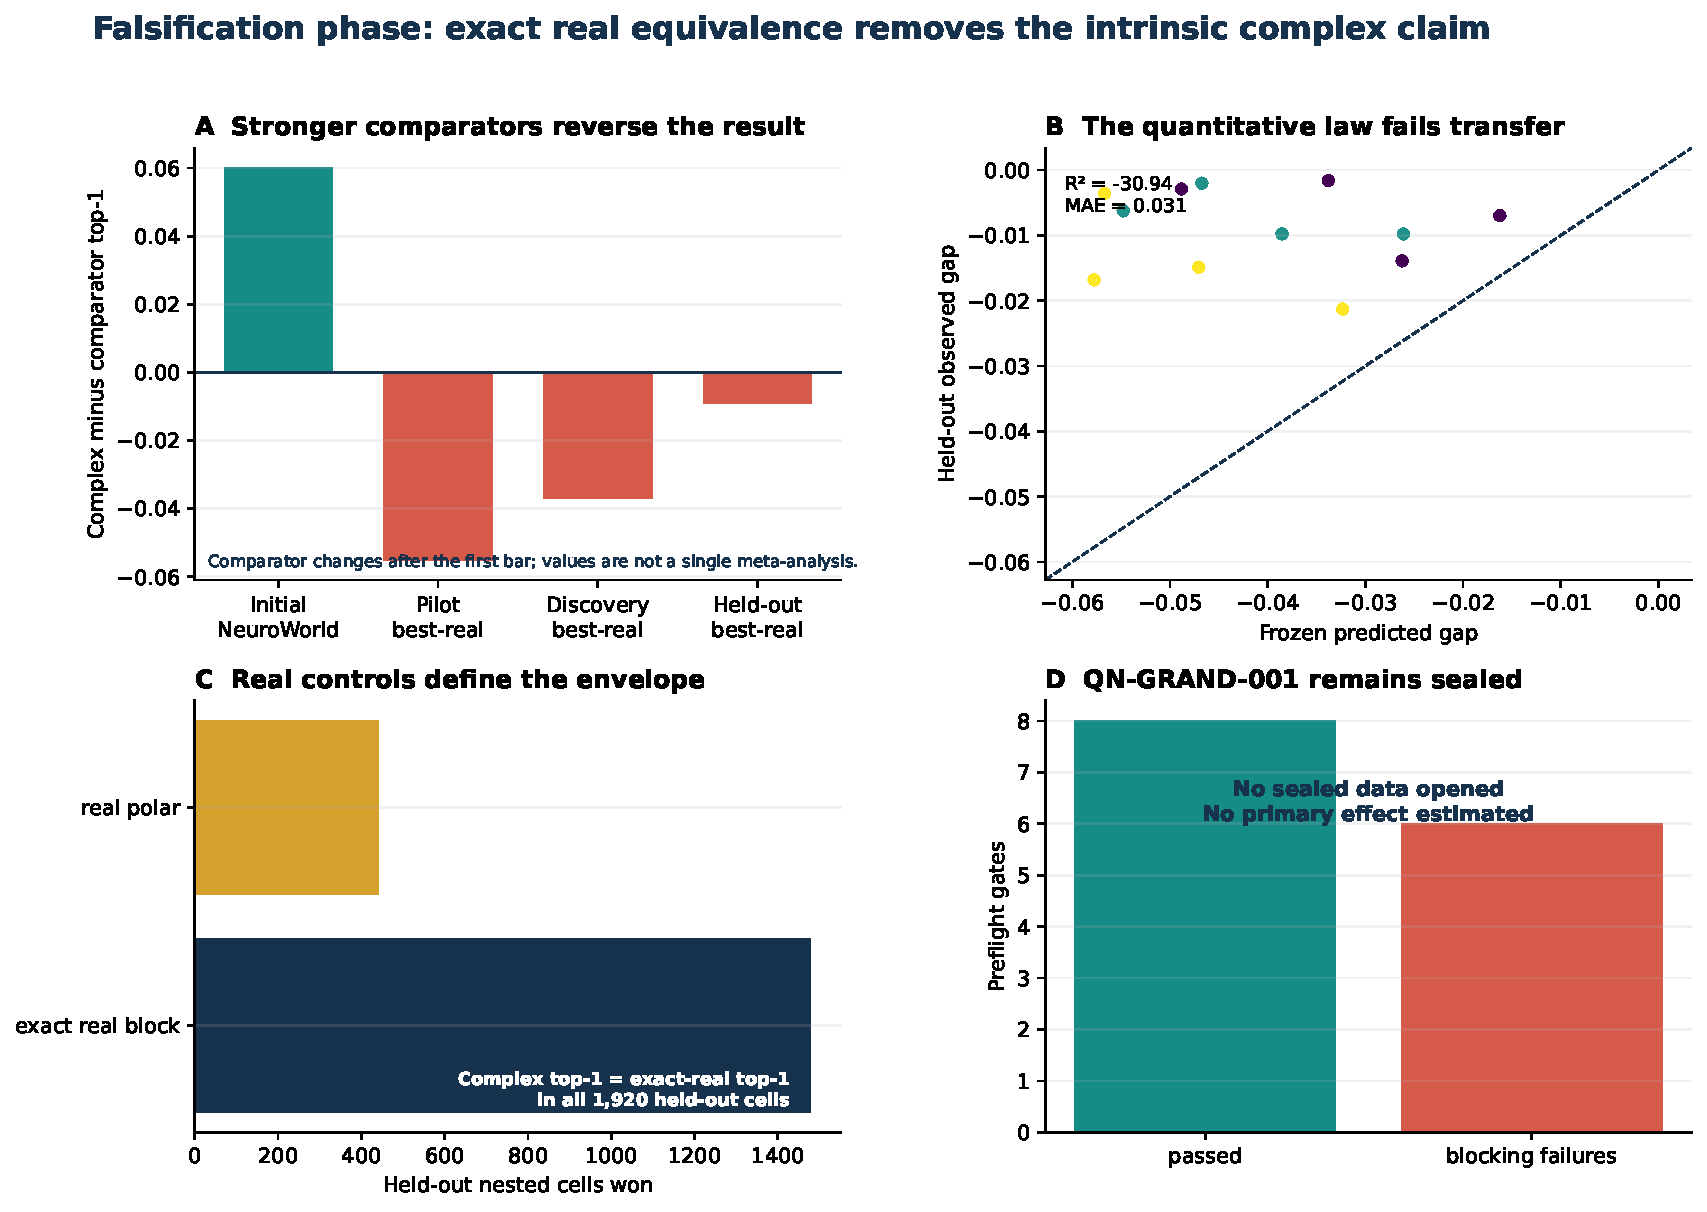
\includegraphics[width=0.98\linewidth]{figures/falsification_phase.pdf}
\caption{Comparator-sensitive effects and prospective stop decisions. The historical positive estimate compares the complex operator with a non-equivalent two-channel real model. Pilot, discovery, and held-out estimates use a best-real envelope that includes the exact block. The held-out interval is a family/world/seed hierarchical bootstrap. The final panel records the failed frozen law and the blocked sealed experiment.}
\label{fig:falsification_phase}
\end{figure}

\subsection{The grand benchmark remains sealed}
QN-GRAND-001 passed eight readiness checks, including the repaired shortcut audit, exact-real equivalence, power planning, frozen-law presence, held-out family separation, and nonmedical scope. It failed six mandatory gates: only 4 of 14 required real controls were present; each evaluated model had one search trial instead of the required 8 or 10; FLOPs and optimizer-step records were missing; the full ShiftGauntlet outcome grid was absent; discovery was reduced rather than full; and raw predictions were not preserved.

The preflight returned \texttt{blocked\_before\_execution}. It records \texttt{executed=false} and \texttt{sealed\_benchmark\_opened=false}, with no primary effect estimate. The stop is a result of the protocol, not an operational accident. Opening the benchmark after a failed gate would convert a prospective test into an exploratory analysis and is deliberately unsupported by the release code.
